\section{COVID19 Supermodel}
\label{sec:covid}
We benchmark our dynamic strategies with the recently introduced COVID supermodel \cite{ansumali2020modelling}, \cite{indiansuper2020supermodel}. This model is a modified SIR model accounting for the possibility of \emph{asymptomatic} patients. These patients can infect susceptible members with a fixed probability. The dynamics account for this new group and its interactions with the traditional SIR groups.

\begin{align}
  \label{eq:covid19_dynamics}
  \begin{split}
   S_A' & = S_A  -(\beta S_A(A+I))\cdot \Delta \\
   S_I' & = S_I  -(\beta S_I (A + I))\cdot \Delta \\
   A' & = A + (\beta S_I(A+I) - \gamma I)\cdot \Delta \\
   I' & = I + (\beta S_I (A+I) - \gamma I)\cdot  \Delta \\
   R_A' & = R_A + (\gamma A)\cdot \Delta \\
   R_I' & = R_I + (\gamma I)\cdot \Delta \\
   D' & = D + (\eta I)\cdot \Delta
  \end{split}
\end{align}
where the variables denote the fraction of a population of individuals designated as \emph{Susceptible to Asymptomatic $(S_A)$}, \emph{Susceptible to Symptomatic $(S_I)$}, \emph{Asymptomatic (A)}, \emph{Symptomatic (I)}, \emph{Removed from Asymptomatic $(R_A)$}, \emph{Removed from Symptomatic $(R_I)$}, and \emph{Deceased (D)}. We choose the parameters ($\beta = 0.25, \gamma=0.02, \eta=0.02$) where $\beta$ is the probablity of infection, $\gamma$ is the removal rate, and $\eta$ is the mortality rate. The parameters are set based on figures shown in \cite{ansumali2020modelling}. The discretization step is chosen to be $\Delta = 0.1$ and the initial box is set to be following dimensions: $S_A  \in [0.69, 0.7], \, S_I \in [0.09, 0.1], \, A \in [0.14, 0.15], \, I \in [0.04, 0.05], \, R_A  = 0,\, R_I  = 0, \, D  = 0$.

Plots of the reachable set for this model tuned to specific values of parameters $\beta, \gamma, \eta$ were published in an ACM Sigbed Blogpost detailing applications of Formal methods for simulating disease dynamics \cite{bak2021covid}.
%
The main theme of the blogpost revolved around the difficulty of extracting accurate parameters from real-world data samples.
%
Certainly we can estimate the parameters by analyzing real-world data. However, minute changes in the parameters could yield estimates which would vastly overestimate or underestimate the true population of infected or asymptomatic patients.
%
This error is further compounded as our time horizon increases due to many of the issues pertaining to wrapping error, as discussed in the Introduction of this thesis (see \ref{sec:intro}).
%
Reachability analysis provides not only a method of simulating the disease dynamics in order to provide meaningful information for policy decisions, but also to demonstrate the effect of slight changes in the parameters on the conservativeness of the outputted reachable set.
%
See Figure \ref{fig:covid_plots} for the two plots published in the blogpost. The Confirmed population is the sum of the number of Symptomatic ($I$) and Asymptomatic ($A$) populations of the dynamics presented in Equation \ref{eq:covid19_dynamics}. The plots were created by dividing the total period into two separate periods.
%
We decided to separate the periods as the parameters presented in the original paper \cite{ansumali2020modelling} were estimated separately according to these exact periods. Furthermore, we wished to control the conservativeness of the over-approximation of the reachable set.
%
The red line represents the real data gathered from India during the prescribed time periods with the light-blue region representing the predicted region based on the parameters given in \cite{ansumali2020modelling}.
%
Several lines representing trajectories generated according to specific parameters are also plotted in order to convey the effect of changes in the population under slight changes of the underlying parameters.
%
\begin{figure}
  \centering
  % First COVID plot.
  \subfloat[Confirmed population from 06/21/20-08/22/20, ]{
    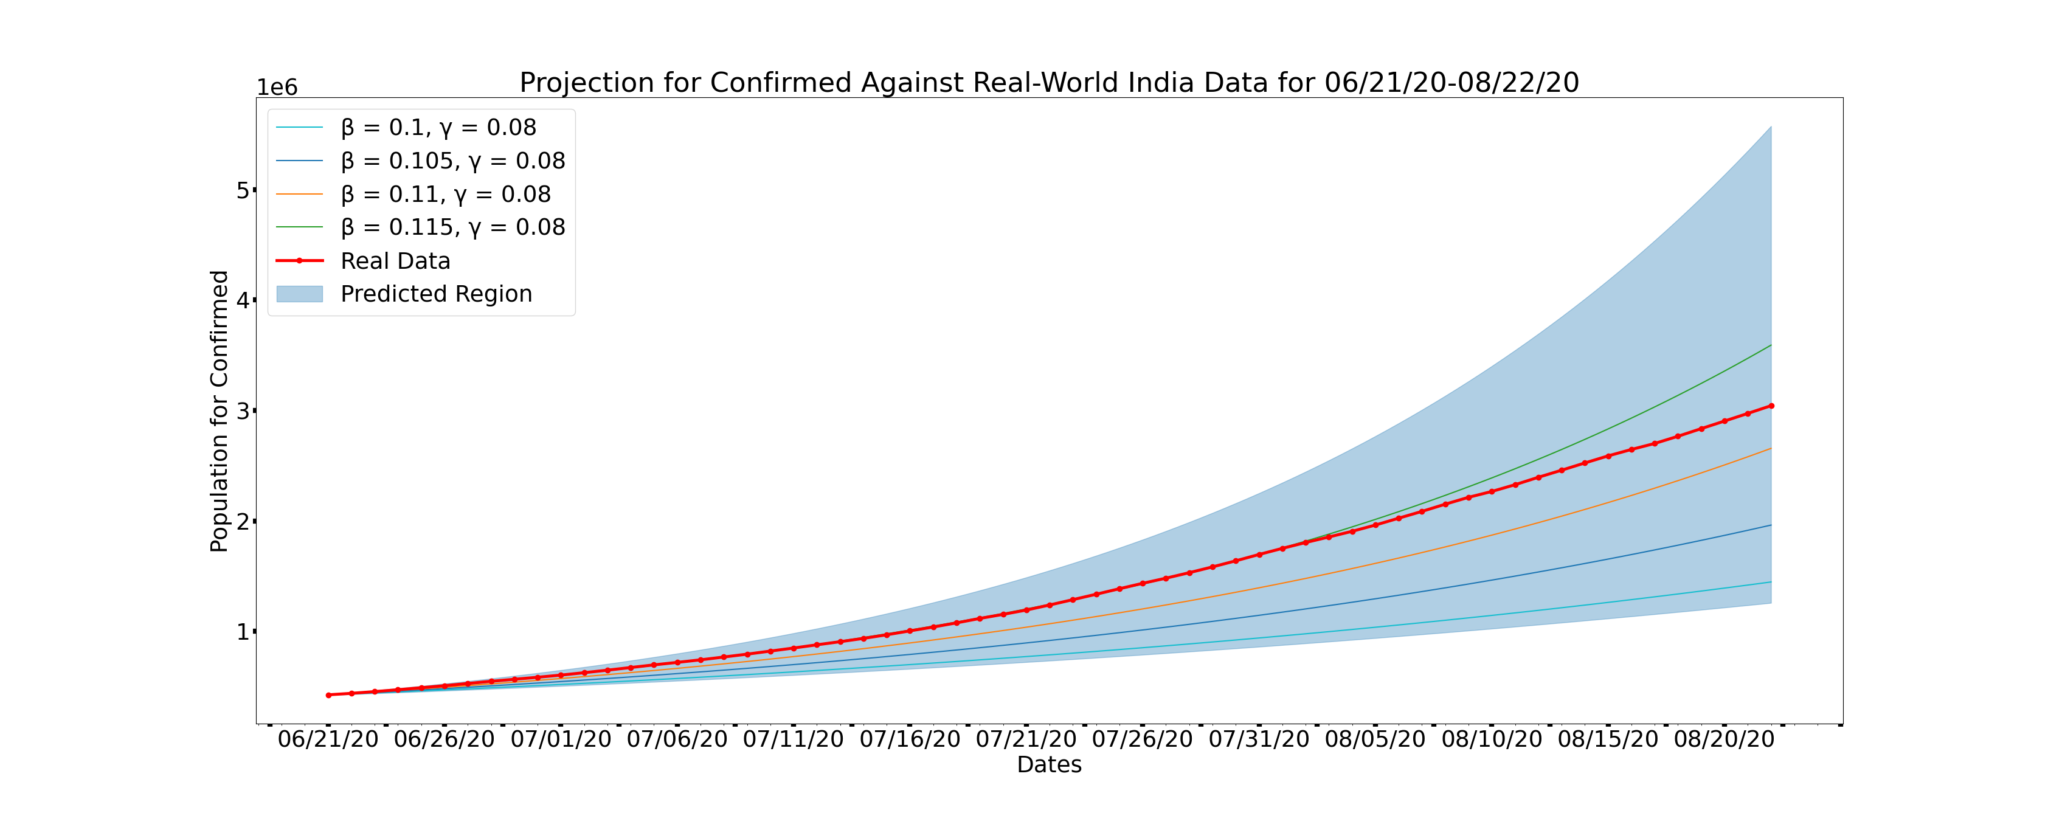
\includegraphics[width= 0.9\textwidth]{figures/IndianRecoveredPlotJun21toAug22-2-2048x813.png}
  }

  \subfloat[Confirmed population from 08/22/20-10/01/20]{
    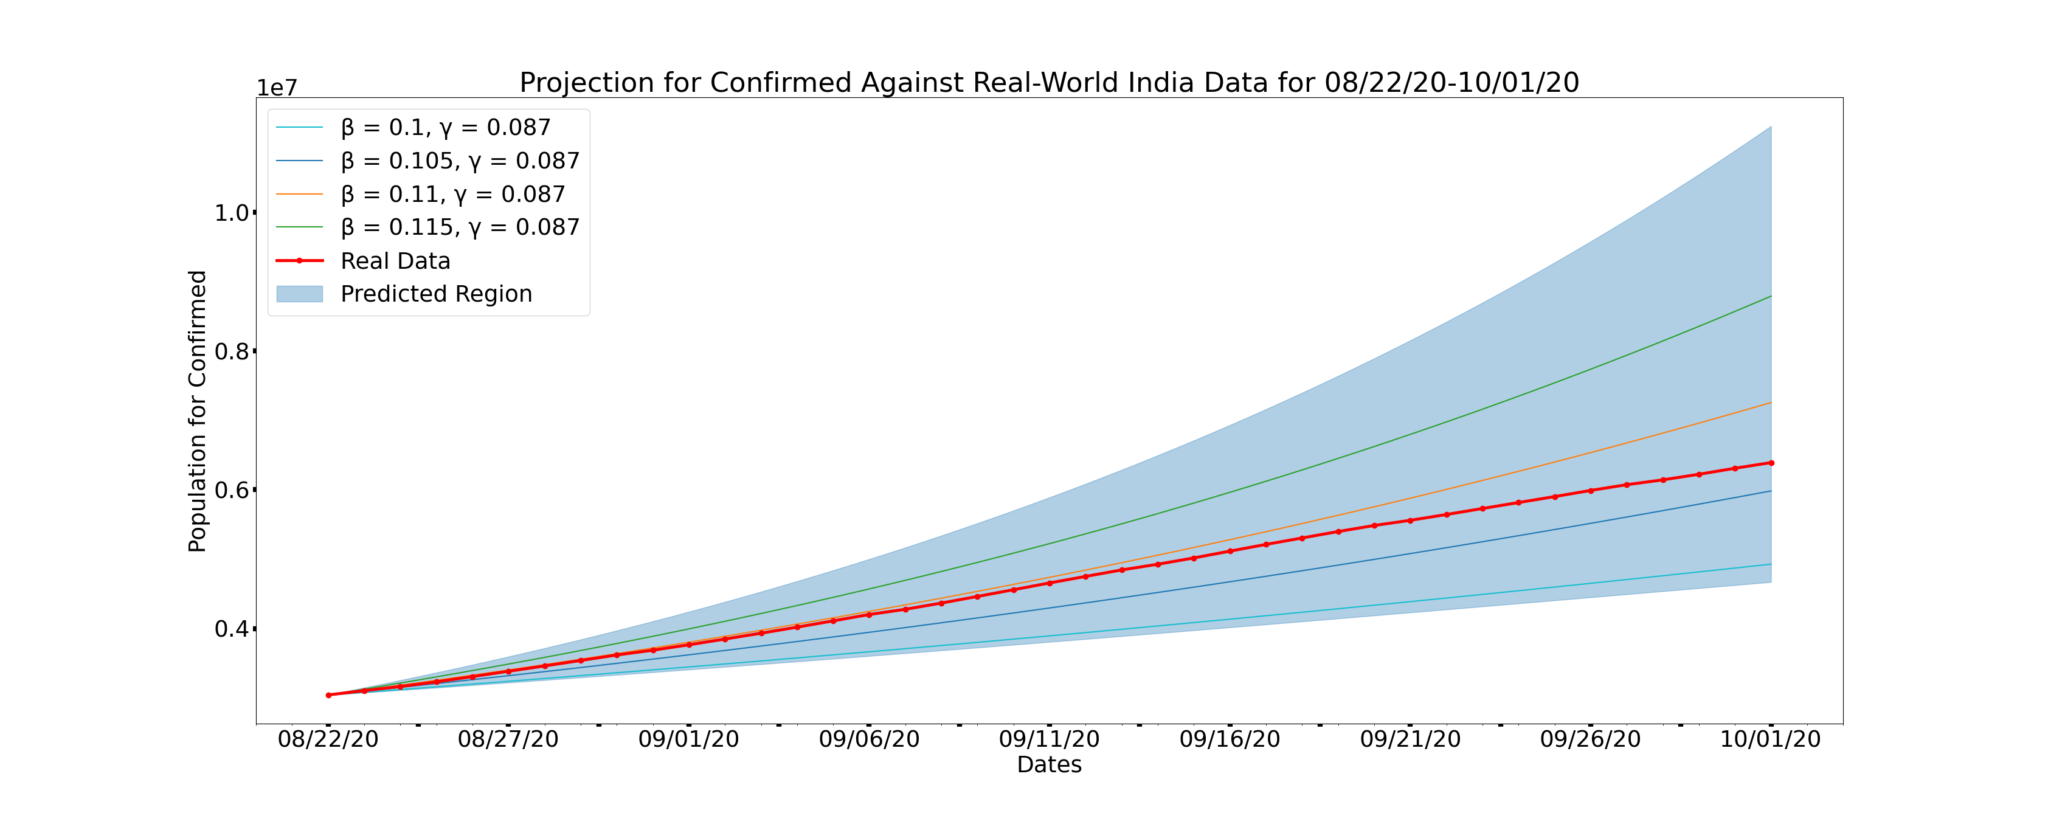
\includegraphics[width= 0.9\textwidth]{figures/IndianRecoveredPlotAug22toOct01-2-2048x813.png}
  }
\caption{Reachable Sets for India's COVID19 Confirmed Population for the period 06/21/20-10/01/20}
\label{fig:covid_plots}
\end{figure}
